\documentclass{report}
\usepackage{graphicx}
\begin{document}
\begin{center}

{\Huge \bf \underline{Semester Diary}}\vspace{1.2in}\\

{\Large by}\\
\vspace{1.2in}
{\Large \bf Prateek Singhal}\vspace{.1in} \\
{\large Y11UC171} \\
\vspace{1.5in}

\includegraphics [width=0.40\textwidth]{lnmiit.jpg}
\end{center}
\pagebreak
{\Huge \bf \underline{Preface}}\vspace{1.5in} \\
\large
\hspace*{1in} I joined The Laxmi Niwas Mittal Institute of Information Technology in 2011 for my Graduation. I am currently a first year B.tech student of Computer Science and Engineering (CSE).\vspace{.5in}\\
\hspace*{1in} In this report known as "Semester Diary" I kept the record of all the activities I did in my first semester. It includes the Academic courses I did,events in which I participated and other happenings that took place in our campus.
\pagebreak
\begin{center} {\Huge \bf \underline{CONTENTS}} \end{center}\vspace{.5in}
\Large
\begin{itemize}
\item \emph{Academics}
\begin{enumerate}
\item Maths - I
\item Physics - I
\item Computer Programming
\item Electronics - I
\item Physics Lab
\end{enumerate}
\item \emph{Extra Curricular activities}
\begin{enumerate}
\item Sports
\item ROOBARU : Freshers party
\item PLINTH : Techno-Management Fest
\item IEEE : Student's chapter
\end{enumerate}
\end{itemize}




\pagebreak
\begin{center}\huge{\bf \underline{Maths - I}}\end{center}\vspace{.3in}
\large \emph{Instructors :}\vspace{.05in}
\begin{itemize}
\item Dr. Akhlaq Husain.
\item Dr. Pratibha Garg.
\end{itemize}
\vspace{.1in}
\emph{Syllabus}:\vspace{.05in}
\begin{itemize}
\item Real numbers, Sequences, Series, Power Series, Limit, Continuity, Differentiability, Mean Value Theorems and applications.
\item Linear approximation, Newton and Picard method, Trapezoidal and Simpson's rule, Error bounds.
\item Taylor's theorem (one variable), Approximation by polynomials, Critical points, Convexity, Curve tracing.
\item Riemann integral, Fundamental theorems of integral calculus, Improper integrals.
\item Space coordinates, Lines and planes, Polar coordinates, Graphs of Polar equations, Cylinders, Quadric Surfaces, Volume, Area, Length.
\item Continuity, Differentiability of vector functions, Arc Length, Curvature, Torsion, Serret‐Frenet formulas.
\item Functions of two or more variables, Partial derivatives. Statement (only) of Taylor's theorem for a function of two variables. Criteria for maxima/minima/saddle points. Applications of maxima/minima for functions of two variables.
\item Multiple integrals: Double, Triple integrals, Fubini's theorem, Jacobians, Surface integrals, Vector calculus, Green, Gauss and Stokes theorem.
\end{itemize}
\vspace{.3in}
\Large{\bf My Grade in Maths - I : \emph{B}}
\pagebreak
\begin{center}\huge{\bf \underline{Physics - I}}\end{center}\vspace{.3in}
\large \emph{Instructors :}\vspace{.05in}
\begin{itemize}
\item Prof. O.P. Katyal.
\item Dr. Anupam Singh.
\item Dr. Amit Neogi.
\end{itemize}
\vspace{.1in}
\emph{Syllabus}:\vspace{.05in}
\begin{itemize}
\item \emph{Mechanics :}
\begin{itemize}
\item Vectors,Kinematics, Plane and Spherical Co-ordinate systems.
\item Force,Newton's laws,Energy,Circular motion,Impulse, Momentum, Collisions.
\item Angular Kinematics,Moment of inertia,Rotational motion,Torque.
\item Central forces,Relativity,Harmonic motion.
\end{itemize}
\item \emph{Thermodynamics :}
\begin{itemize}
\item Systems,Equations of States,Laws of Thermodynamics.
\item Turbine, Compressor,Boiler,Nozzle,Throttle,Condenser,Refrigerator.
\item Heat engine,Temperature Scale,Carnot Cycle.
\end{itemize}
\item \emph{Optics :}
\begin{itemize}
\item Historical Development of optics,Mechanical,Plane,Electromagnetic Waves.
\item Poynting Vector,Superposition of waves,standing waves,Resonance.
\item Lasers,Interference,Wavefront,Newton's rings.
\end{itemize}
\end{itemize}
\vspace{.3in}
\Large{\bf My Grade in Physics - I : \emph{A}}
\pagebreak
\begin{center}\huge{\bf \underline{Computer Programming}}\end{center}\vspace{.3in}
\large \emph{Instructor :}\vspace{.1in}\\
\hspace*{.1in} Subrat Kumar Dash.\vspace{.1in}\\
\emph{Syllabus}:\vspace{.05in}
\begin{itemize}
\item Introduction to Problem Solving,Flow charts, Tracing flow charts,Sample Programs written in C .
\item Identifiers and keywords, Data types, Declarations, Expressions, statements. 
\item Operators and expressions: Arithmetic, unary, logical, bit-wise, assignment and conditional operators
\item While, do-while, for statements, nested loops, if else, switch, break, Continue, and goto statements,comma operators 
\item Storage class: Automatic, external, register and static variables. 
\item Functions: Defining and accessing, passing arguments, Function prototypes, Recursion, Library 
functions, Static functions.
\item Arrays: Defining and processing, Passing arrays to a function, Multi dimensional arrays. 
\item Strings: Defining and operations on strings. 
\item Pointers:Declarations, Passing pointers  to a function, Operations on  pointers, Pointer Arithmetic, 
Pointers and arrays, Arrays of pointers function pointers. 
\item Structures:Defining and processing, Passing to a function,  Unions, typedef, array of structure, and 
pointer to structure. 
\item File operation: creation, copy, delete, update, text file, binary file. 
\end{itemize}
\Large{\bf My Grade in Computer Programming : \emph{A}}
\pagebreak
\begin{center}\huge{\bf \underline{Electronics - I}}\end{center}\vspace{.3in}
\large \emph{Instructor :}\vspace{.1in}\\
\hspace*{.1in} Dr. Soumitra Debnath.\vspace{.1in}\\
\emph{Syllabus}:\vspace{.05in}
\begin{itemize}
\item \emph{Network Analysis}:
\begin{itemize}
\item Kirchoff's Law,Thevenin and Norton Theorem,Superposition Theorem.
\item Complex Frequency, R-L,R-C,R-L-C, Circuits,Power Factor,Complex Power.
\item Laplace Transform,Frequency Response,Bode plots,Star-Delta,Cramer's Rule.
\end{itemize}
\item \emph{Op - Amp}:
\begin{itemize}
\item Positive,Negative Feedback,Inverting, Non inverting Amplifiers,Voltage Follower,Loading effect.
\item Difference,Summing,Integrator,Differentiator Amplifiers,temperature Sensor.
\item Schimitt trigger, Oscillators.
\end{itemize}
\item \emph{Digital Circuits}:
\begin{itemize}
\item Number systems: Binary, Octal, Decimal, Hexadecimal
\item Complements,Boolean algebra,Logic Gates,Truth Tables.
\item AND,OR,NOT,XOR,XNOR,NOR,NAND gates.
\item POS,SOP,K-Map,Half Adder,Full Adder,BCD to 7 segment display.
\item Sequential Circuits,Comparators,Decoder,Encoder,Multiplexer,Flip-Flops,Counters.
\end{itemize}
\end{itemize}
\Large{\bf My Grade in Electronics - I : \emph{B}}
\pagebreak
\begin{center}\huge{\bf \underline{Physics Lab}}\end{center}\vspace{.3in}
\large \emph{Instructors :}\vspace{.05in}
\begin{itemize}
\item Prof. O.P. Katyal.
\item Somnath Biswas.
\item Dr. Amit Neogi.
\end{itemize}
\vspace{.1in}
\emph{Experiments}:\vspace{.05in}
\begin{itemize}
\item Introduction to measurement and analysis,Significant Figures,Error analysis.
\item Moment of inertia of Wheel, Bar Pendulum.
\item Fraunhofer Diffraction,Refractive Index of a Prism.
\item Helmholtz Coil, Demonstration of eddy Currents.
\item Phase velocity of Rope Waves,Adiabatic Module for Climate simulation.
\item Gyroscope,Forced Damped Oscillations in LCR Circiuts.
\item Current Balance and Force acting on a current carrying Conductor.
\item Electromagnetic Induction,Dependence of hall Coefficient on Temperature.
\item Diffraction Grating, Measurement of Resistivity and Band gap of a semi conductor using four probe method.
\end{itemize}
\Large{\bf My Grade in Physics Lab : \emph{B}}
\pagebreak
\begin{center}\huge{\bf \underline{Sports}}\end{center}
\vspace{1in}
\hspace{.5in} The LNMIIT campus is provided with all the sports facilities. We have got Volley ball, Badminton, Table tennis,Football,Cricket,Basket Ball,etc. During my school life i was not very active in sports activities but after coming to The LNMIIT I got nice exposure to sports. I used to play badminton and table tennis.
\vspace{.5in}
\begin{center}
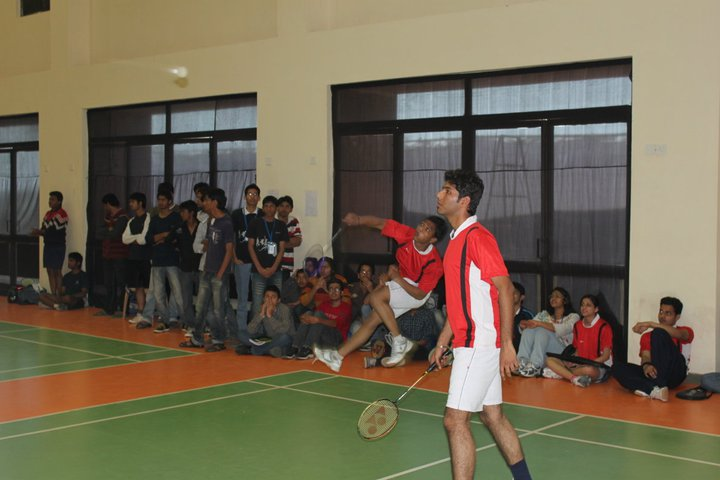
\includegraphics [width=0.40\textwidth]{baddy.jpg}\vspace{.5in}\\
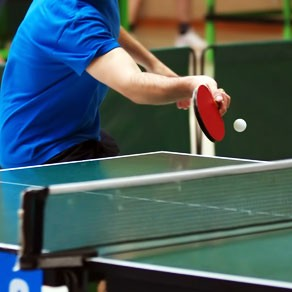
\includegraphics [width=0.40\textwidth]{tt.jpg}
\end{center}
\pagebreak
\begin{center}\huge{\bf \underline{Roobaroo '11}}\end{center}
\vspace{.15in}
\hspace{.5in} Roobaroo '11 was the freshers party of the Y11 batch. It was celebrated with great pump and show with the following events :
\begin{itemize}
\item Drama
\item Dance and Music
\item Fun activities like \emph{Ice Break}
\item Rock Band Performance
\end{itemize}
\vspace{.5in}
\begin{center}
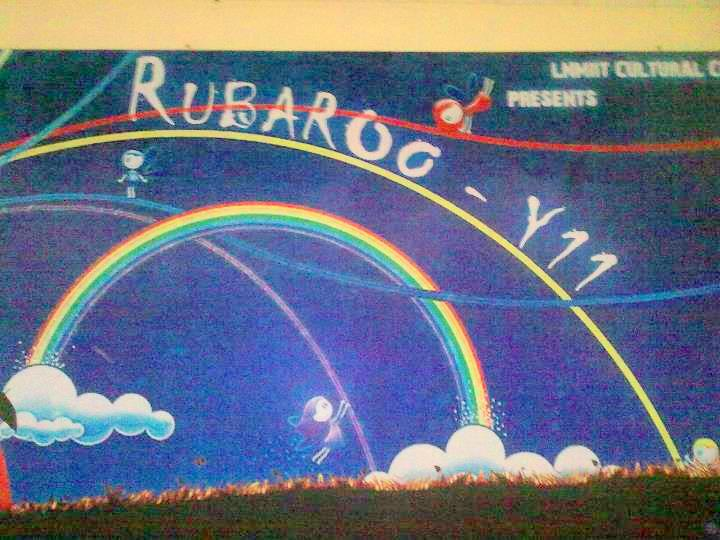
\includegraphics [width=0.40\textwidth]{p1.jpg}\hspace{.5in}
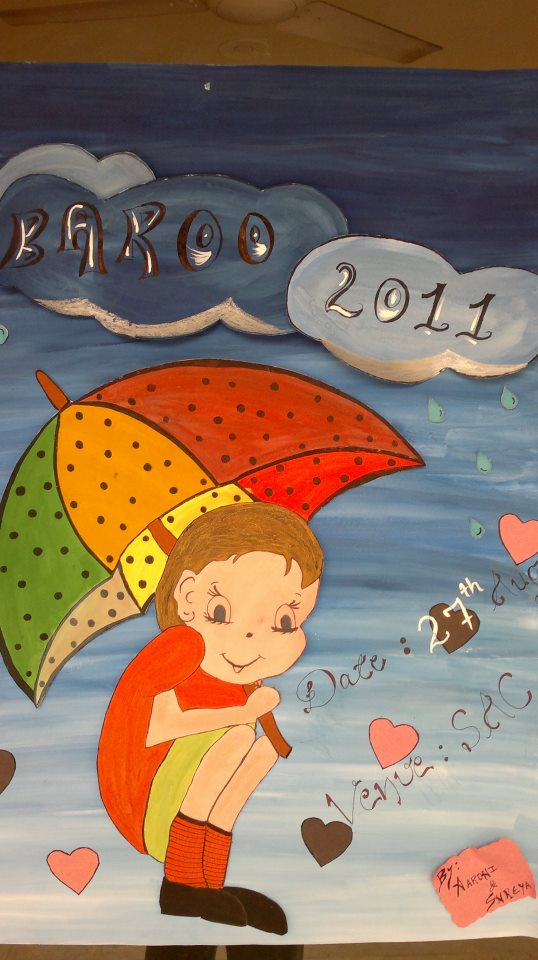
\includegraphics [width=0.30\textwidth]{p2.jpg}
\end{center}
\pagebreak
\begin{center}\huge{\bf \underline{Plinth '11}}\end{center}
\vspace{.15in}
\hspace{.5in} Plinth '11 was the Techno-Management Fest. The following events are the key attractions of this event.

\begin{itemize}
\item Robotics
\begin{itemize}
\item Robo race

\item Robo Soccer

\item Robo war
\item Line Follower
\end{itemize}
\item Cyber events
\begin{itemize}
\item Prison Break
\item IUPC

\item OS Mania
\end{itemize}
\item Management
\begin{itemize}
\item Cell with E-Cell
\item Ad-Mad
\item B-Plan
\item Economic Debate
\end{itemize}
\end{itemize} 
\paragraph{\LARGE{I participated in IUPC-Intra University Programming Contest and secured 5th position.}}

\vspace{1in}
\begin{center}\huge{\bf \underline{IEEE Students Chapter '11}}\end{center}
\vspace{.15in}
\begin{center}
\hspace{.5in} IEEE students  chapter was introduced in The LNMIIT last year. It inspires the students toward Reasearch in the enginneering field. Many International level Conferences and Workshops are organised under the IEEE Students chapter at our campus like that of HTML5,Android,Microwaves,etc.
\vspace{.5in}\\

\includegraphics [width=0.50\textwidth]{p5.jpg}
\vspace{.5in}\\
 IEEE as a society is more popular for the volunteerism opportunities it provides to every individual member starting from the student member grade to fellow grade. 
\emph{I also volunteered for the IEEE workshop organised by W3C India on HTML 5}
\end{center}










\end{document}